\chapter{Versuchsaufbau}
\section{Einleitung}

\begin{figure}[H]
    \centering
    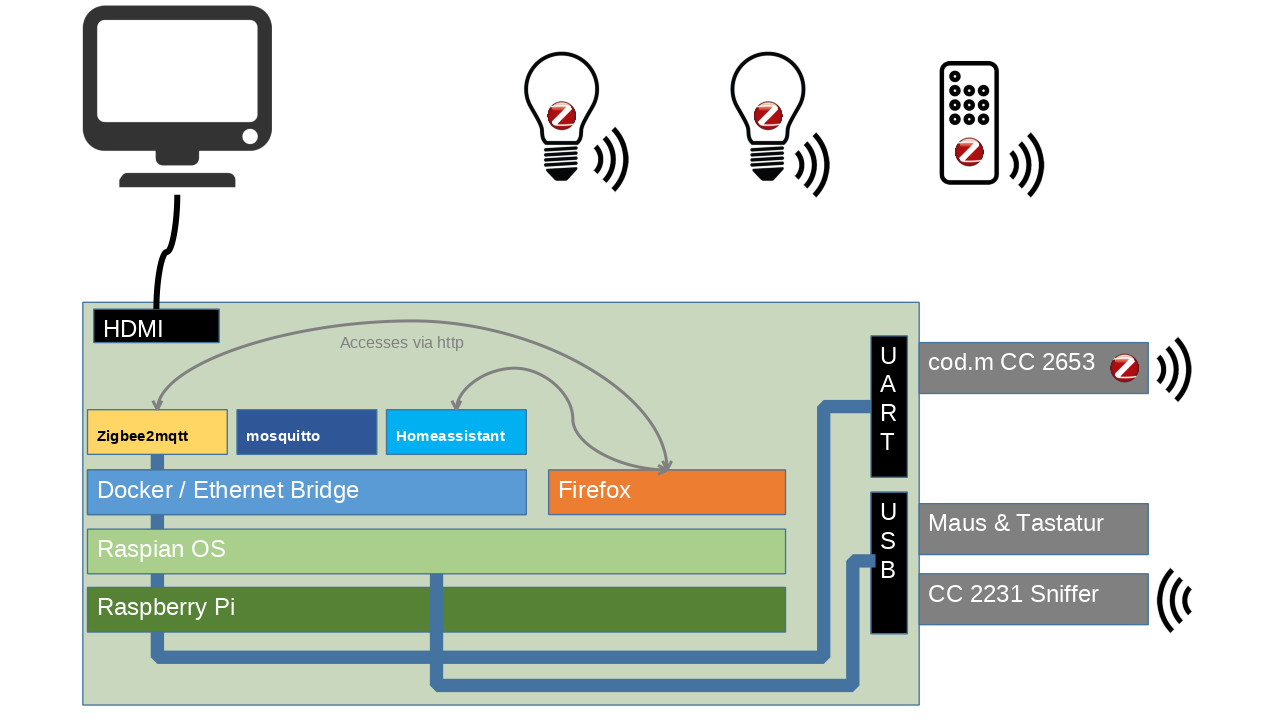
\includegraphics[width=1\textwidth]{media/Versuchsaufbau/image1.png}
    \caption{Versuchsaufbau}
  \end{figure}

In dieser Abbildung wird der schematische Versuchsaufbau gezeigt. Die drei Anwendungen werden als Docker Container ausgeführt. Sie kommunizieren
untereinander über ein eigenes Docker Netzwerk. Dies ist eine von Docker verwaltete Linux Bridge. Nur der NGINX Reverse Proxy hat zwei Ports die
auf die Host Schnittstelle gebunden werden. Die Webfrontends sind damit über den lokal installierten Browser über das Loopback-Interface erreichbar. 
Damit ist der Raspberry Applikationsserver und Versuchs-PC zugleich.

Es werden entsprechende Namen in der lokalen \grqq hosts\grqq{} Konfigurationsdatei hinterlegt, um lokal Domainnamen auflösen zu können.

Der cod.m Zigbee Controller wird direkt an den Docker Container durchgereicht. Der Sniffer Stick ist regulär am Host angeschlossen. 

\section{Containerverwaltung}



\subsection{Nginx Proxy}
\begin{lstlisting}
    proxy:
      container_name: nginx
      image: jwilder/nginx-proxy:alpine
      networks:
        - backbone
      ports:
        - 80:80
        - 443:443
      volumes:
        - ./NGINX/proxy/conf.d:/etc/nginx/conf.d:rw
        - ./NGINX/proxy/vhost.d:/etc/nginx/vhost.d:rw
        - ./NGINX/proxy/html:/usr/share/nginx/html:rw
        - ./NGINX/proxy/certs:/etc/nginx/certs:ro
        - /etc/localtime:/etc/localtime:ro
        - /var/run/docker.sock:/tmp/docker.sock:ro
      restart: unless-stopped
\end{lstlisting}

Der Proxy basiert auf einem Image des Proxys NGINX \cite{nginxpm}. Vorteil dieses erweiterten NGINX ist es,
dass dieser automatisiert seine Konfigurationen verwaltet. Dafür wird bei einem Service eine Umgebungsvariable gesetzt. Über den 
\grqq docker.sock\grqq{} erfährt der Proxy ob Container gestartet werden und kann auf deren Umgebungsvariablen zugreifen. Wird ein Container mit der Umgebungsvariable 
\grqq VIRTUAL\_HOST=z2m.local \grqq{} gestartet, wird automatisch eine Weiterleitung für alle Anfragen mit dem Header \grqq z2m.local\grqq{} auf den Container eingerichtet.
Alle Servicecontainer sind in einer eigenen L2-Domäne und von außen nicht direkt erreichbar. Der Proxy Container ist der einzige, dem externe Ports zugewiesen werden.
Dies wird durch entsprechende \grqq iptables\grqq{} Einträge umgesetzt.

\begin{figure}[H]
  \centering
  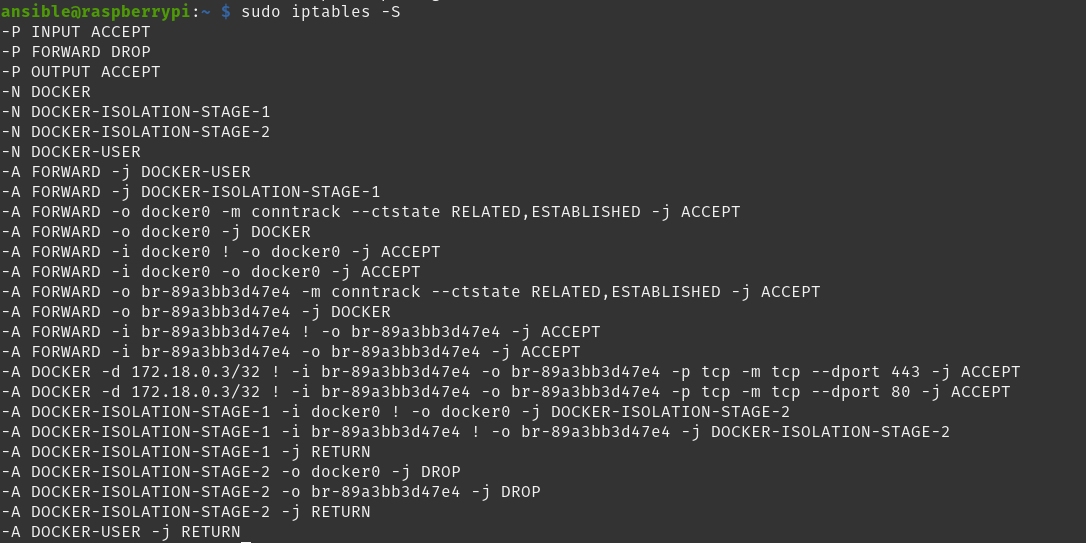
\includegraphics[width=1\textwidth]{media/rasp-iptables.png}
  \caption{Raspberry iptables}
\end{figure}
Die Regeln in der Tabelle \grqq DOCKER \grqq{} werden durch Docker geschrieben. Eigene Regeln können in der Tabelle 
\grqq DOCKER-USER \grqq{} definiert werden.

\begin{figure}[H]
  \centering
  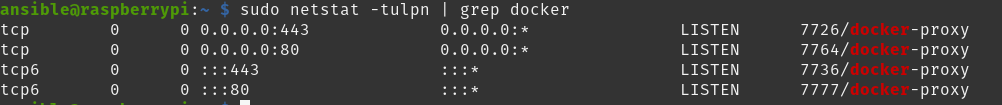
\includegraphics[width=1\textwidth]{media/rasp-netstat.png}
  \caption{Raspberry netstat}
\end{figure}
In dieser Ausgabe ist erkennbar, dass Docker auf die Ports 80 und 443 lauscht.

\subsection{zigbee2mqtt}
\begin{lstlisting}
  zigbee2mqtt:
    container_name: zigbee2mqtt
    image: koenkk/zigbee2mqtt
    networks:
      - backbone
    volumes:
      - ./Z2M/data:/app/data
    devices:
       - /dev/ttyAMA0:/dev/ttyAMA0
    restart: always
    environment:
      - VIRTUAL_HOST=z2m.local
      - VIRTUAL_PORT=8080
    group_add:
      - dialout
\end{lstlisting}

Dem Container wird ebenfalls das Netzwerk \grqq backbone\grqq{} zugewiesen. Ein Verzeichnis mit Konfigurationen und persistenten Datensätzen wird auf den Host gemountet. Wenn der gemountete Pfad außerhalb des Containers nicht existiert, wird der 
bestehende Ordner aus dem Container kopiert. Existiert der Pfad, wird der Ordner vom Host in den Container gemountet. 
Bei Linux können Geräte über das selbe Verfahren wie Verzeichnisse adressiert werden. \grqq - /dev/ttyUSB0:/dev/ttyACM0\grqq{} reicht den ZigBee Adapter an 
den Docker Container weiter.
In den Umgebungsvariablen wird dem Proxy noch mitgeteilt, unter Welcher URL er erreichbar sein soll und auf welchem Port der Webserver läuft. Die Gruppe 
\grqq dialout\grqq{} ist notwendig, damit der Container Zugriffsrechte auf die serielle Schnittstelle des Hosts erhält.

Die zentrale Konfigurationsdatei von Zigbee2mqtt:
\begin{lstlisting}
homeassistant: true
permit_join: false
mqtt:
  base_topic: zigbee2mqtt
  server: mqtt://mosquitto:1883
serial:
  port: /dev/ttyACM0
frontend:
  port: 8080
  host: 0.0.0.0
  url: https://z2m.local
advanced:
  homeassistant_legacy_entity_attributes: false
  legacy_api: false
  legacy_availability_payload: false
device_options:
  legacy: false
\end{lstlisting}

Es wird der \grqq Homeassistant\grqq{} Modus aktiviert, Damit werden die Nachrichten an den MQTT Broker für Homeassistant verständlich gestaltet.
Das Beitreten neuer Geräte ist standardmäßig deaktiviert und muss explizit erlaubt werden. Des Weiteren wird ein MQTT Server angegeben, sowie ein \grqq base-topic\grqq{}
definiert. Docker löst Containernamen in Docker Netzwerken zu IP-Adressen auf, sodass hier als Server der entsprechende Containernamen angegeben werden
kann. Im weiteren wird der Pfad angegeben, auf den der cod.m Adapter gemountet wurde, sowie entsprechende Einstellung für den Webserver gesetzt.

\subsection{mosquitto}

\begin{lstlisting}
  mosquitto:
  container_name: mosquitto
  image: eclipse-mosquitto:latest
  networks:
    - backbone
  restart: always
  deploy:
    resources:
      limits:
        memory: 125M
  volumes:
    - ./mosquitto/config:/mosquitto/config
    - ./mosquitto/data:/mosquitto/data
    - ./mosquitto/log:/mosquitto/log
\end{lstlisting}

Als MQTT Broker wird \grqq mosquitto\grqq{} eingesetzt. Die Konfigurationen 
wurden auch hier entsprechend auf den Host gemountet. Als Konfigurationsdatei wird das Standardtemplate verwendet, welches nur an zwei 
entsprechenden Stellen modifiziert ist.

\begin{lstlisting}
... 
allow_anonymous true
... 

... 
listener 1883
... 
\end{lstlisting}

Es wird der Zugriff von nicht authentifizierten Geräten erlaubt. Dies stellt kein Risiko dar, da der Container nur innerhalb des \grqq backbone\grqq{} 
Netzwerkes sowie vom Host selber erreichbar ist. Zusätzlich wird der Port definiert, auf dem der MQTT Service läuft. 1883 ist der standard Port für MQTT.

\section{Namensauflösung}

Für eine lokale Namensauflösung werden die Hosts in die \grqq \textbackslash etc\textbackslash hosts\grqq{} eingetragen. Dies wird automatisch in der Ansible
Rolle \grqq DeployLab\grqq{} gemacht.

\begin{lstlisting}
- name: Add Hosts Entrys
  become: True
  lineinfile:
    path: /etc/hosts
    line: 127.0.0.1 z2m.local
\end{lstlisting}

\section{Anwendungen}

Für den Versuch wird weiterhin ein Webbrowser sowie Wireshark benötigt. Die beiden Anwendungen werden per Ansible installiert:
\begin{lstlisting}
  - name: Install required Packages
  become: true
  apt:
    pkg:
      - wireshark
      - firefox
    state: latest
    update_cache: true
\end{lstlisting}

Die Konfigurationen der Anwendungen werden per Ansible überschrieben. Ebenso wird die Binärdatei die zur Anbindung des Sniffersticks als externes Interface an Wireshark benötigt wird 
per Ansible implementiert. In Wireshark ist zu Beginn das Layout auf ZigBee angepasst. Zusätzlich sind die notwendigen Schlüssel zum Entschlüsseln der Kommunikation eingetragen. Unter 
dem Protokoll IEEE 802.15.4 ist ebenfalls das FCS Formart auf TI CC24XX gestellt. Ansonsten werden die Pakete als Fehlerhaft markiert und nicht korrekt dargestellt.

\begin{figure}[H]
  \centering
  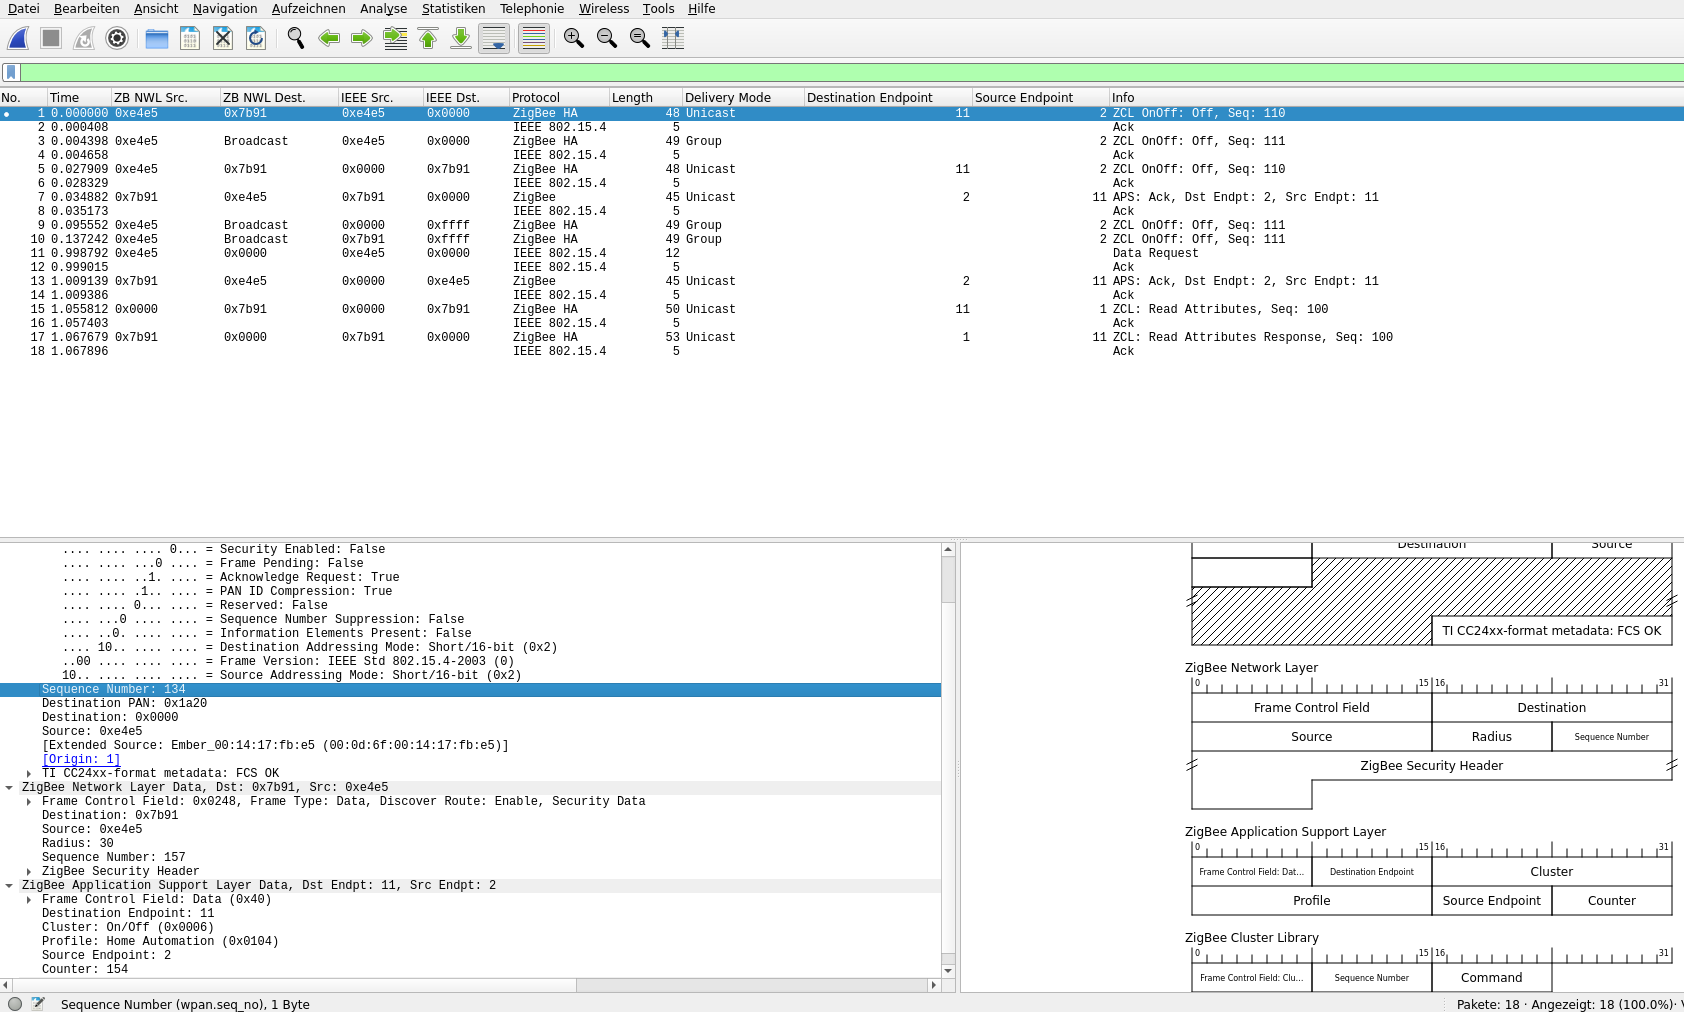
\includegraphics[width=1\textwidth]{media/ws-configured.png}
  \caption{Wireshark mit angepassten Layout}
\end{figure}

In dem Layout sind werden direkt die Adressen aus dem IEEE Layer und dem ZigBee NWL Layer dargestellt. Damit ist immer das Ziel sowie der aktuelle Hop direkt erkennbar.

\section{Devices}

Als Zigbee Devices kommen folgende Geräte zum Einsatz:

\begin{itemize}
  \item Phillips Hue Dimmer Switch V1
  \item 2 x Phillips Hue White A60 E27
  \item cod.m RaspberryPi Hat
\end{itemize}

\subsection{Fernbedienung}
Als Alternative zur Phillips Hue Fernbedienung wurde ein OSRAM Lightify Switch Mini getestet. Die Phillips Hue Fernbedienung hat den Nachteil,
das ein Hardreset nur über einen Knopf auf der Rückseite, welcher per Büroklammer oder ähnlichem betätigt werden muss, möglich ist. Nur nach diesem 
Hardreset erlaubt die Fernbedienung eine neue PAN-ID und sucht auf anderen Kanälen nach verfügbaren Netzwerken. Die Erfahrung zeigt allerdings,
dass dieser Reset Taster nicht sonderlich standhaft ist und gerade im Praktikumsbetrieb schnell verschleißt. Ebenso ist ein Softreset möglich,
indem alle Tasten der Fernbedienung gleichzeitig gedrückt werden. Allerdings bleibt hier die Konfiguration persistent, und es wird nur einem 
vorher bekannten Netzwerk neu beigetreten. 

Weiteres Manko sind proprietäre Funktionen von Phillips Hue. So werden Kommandos verschickt, die nicht im Standard enthalten sind und lediglich von der Phillips Hue Bridge verstanden 
werden können \cite{koe}. Weiterhin setzen Phillips und viele weitere Herstelle das ZigBee Binding nicht in Ihren Ecosystemen ein. Die Logik, welche Lampe durch 
die Fernbedienungstasten gesteuert werden, ist in die Hue Bridge implementiert. Das Binding ist damit oft nur mangelhaft implementiert. Der Dimmer Switch 
zeigt oft das Verhalten seine Bindings nicht mehr zu aktualisieren, obwohl neue Binding Requests bestätigt werden. In Wireshark erkennt man, das alle Kommandos
an eine nicht vorhandene Gruppe geschickt werden zum Beispiel. Dieses Fehlerbild ist nur mit einem Hardreset lösbar. 

Die Osram Fernbedienung ist haptisch deutlich ansprechender als die Phillips Fernbedienung. Zusätzlich lässt sich diese per Tastenkombinationen auf der 
Vorderseite Softreseten, Hardreseten sowie in den Pairingmodus schalten. In diesem Modus tritt sie zuverlässig neuen Netzwerken bei und verhielt sich 
deutlich unkomplizierter als die Phillips Hue Fernbedienung. 

Leider hat die Implementation des Bindings erhebliche Mängel und ist damit nicht nutzbar. Auch hier werden alle Bindungsanfragen von Zigbee2Mqtt zuverlässig 
bestätigt. Die Fernbedienung bietet 3 Endpunkte, die allesamt einzeln Problemfrei gebunden werden können. Auch hier führt allerdings ein doppeltes Binding auf einem 
Endpunkt zu inkonsistentem Verhalten. Es lässt sich also pro Endpunkt nur ein Device Binden.

Leider verhält sich die Fernbedienung nur beim drücken des \grqq Off\grqq Buttons korrekt. Bei dem \grqq On\grqq Button verschickt die Fernbedienung die Kommando Frames immer 
per Broadcast. Dies führt bei großen Netzwerken dazu, dass alle Geräte sich einschalten. Die beiden Buttons gehören zum selben Cluster und Bindings gelten pro Cluster. Daher ist 
dieses Verhalten nicht nachvollziehbar. Auch hier wird Osram die Funktion in seinem Ecosystem entweder überhaupt nicht einsetzen und es ist irrelevant das die Funktion nicht korrekt 
umgesetzt ist, oder sie haben eine eigene Logik die keinem Standard entspricht und das Binding entsprechend modifiziert.

\begin{figure}[H]
  \centering
  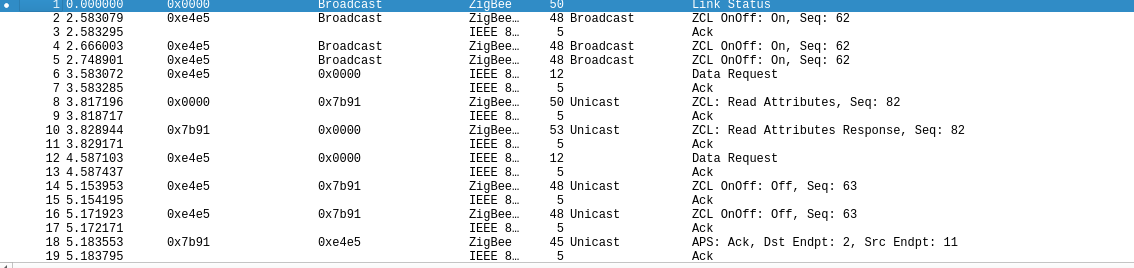
\includegraphics[width=1\textwidth]{media/osram-device.png}
  \caption{Osram Bug - Binding mit Device}
\end{figure}
Hier ist zu sehen wie die Off-Nachricht per Unicast korrekterweise an die Lampe verschickt wird. Die On-Nachricht wird allerdings an die Broadcast Adresse geschickt.

\begin{figure}[H]
  \centering
  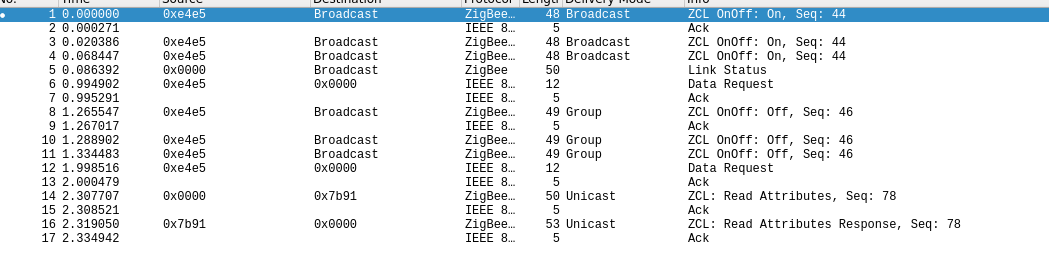
\includegraphics[width=1\textwidth]{media/osram-group.png}
  \caption{Osram Bug - Binding mit Group}
\end{figure}
Das identische Verhalten ist bei einem Binding mit einer Gruppe zu beobachten.

